% Figure Captions for Partition Lagrangian Paper
% Generated from partition_lagrangian_figures.py visualization suite

%==============================================================================
% Figure 1: Partition Lagrangian Dynamics
%==============================================================================
\begin{figure*}[!htbp]
    \centering
    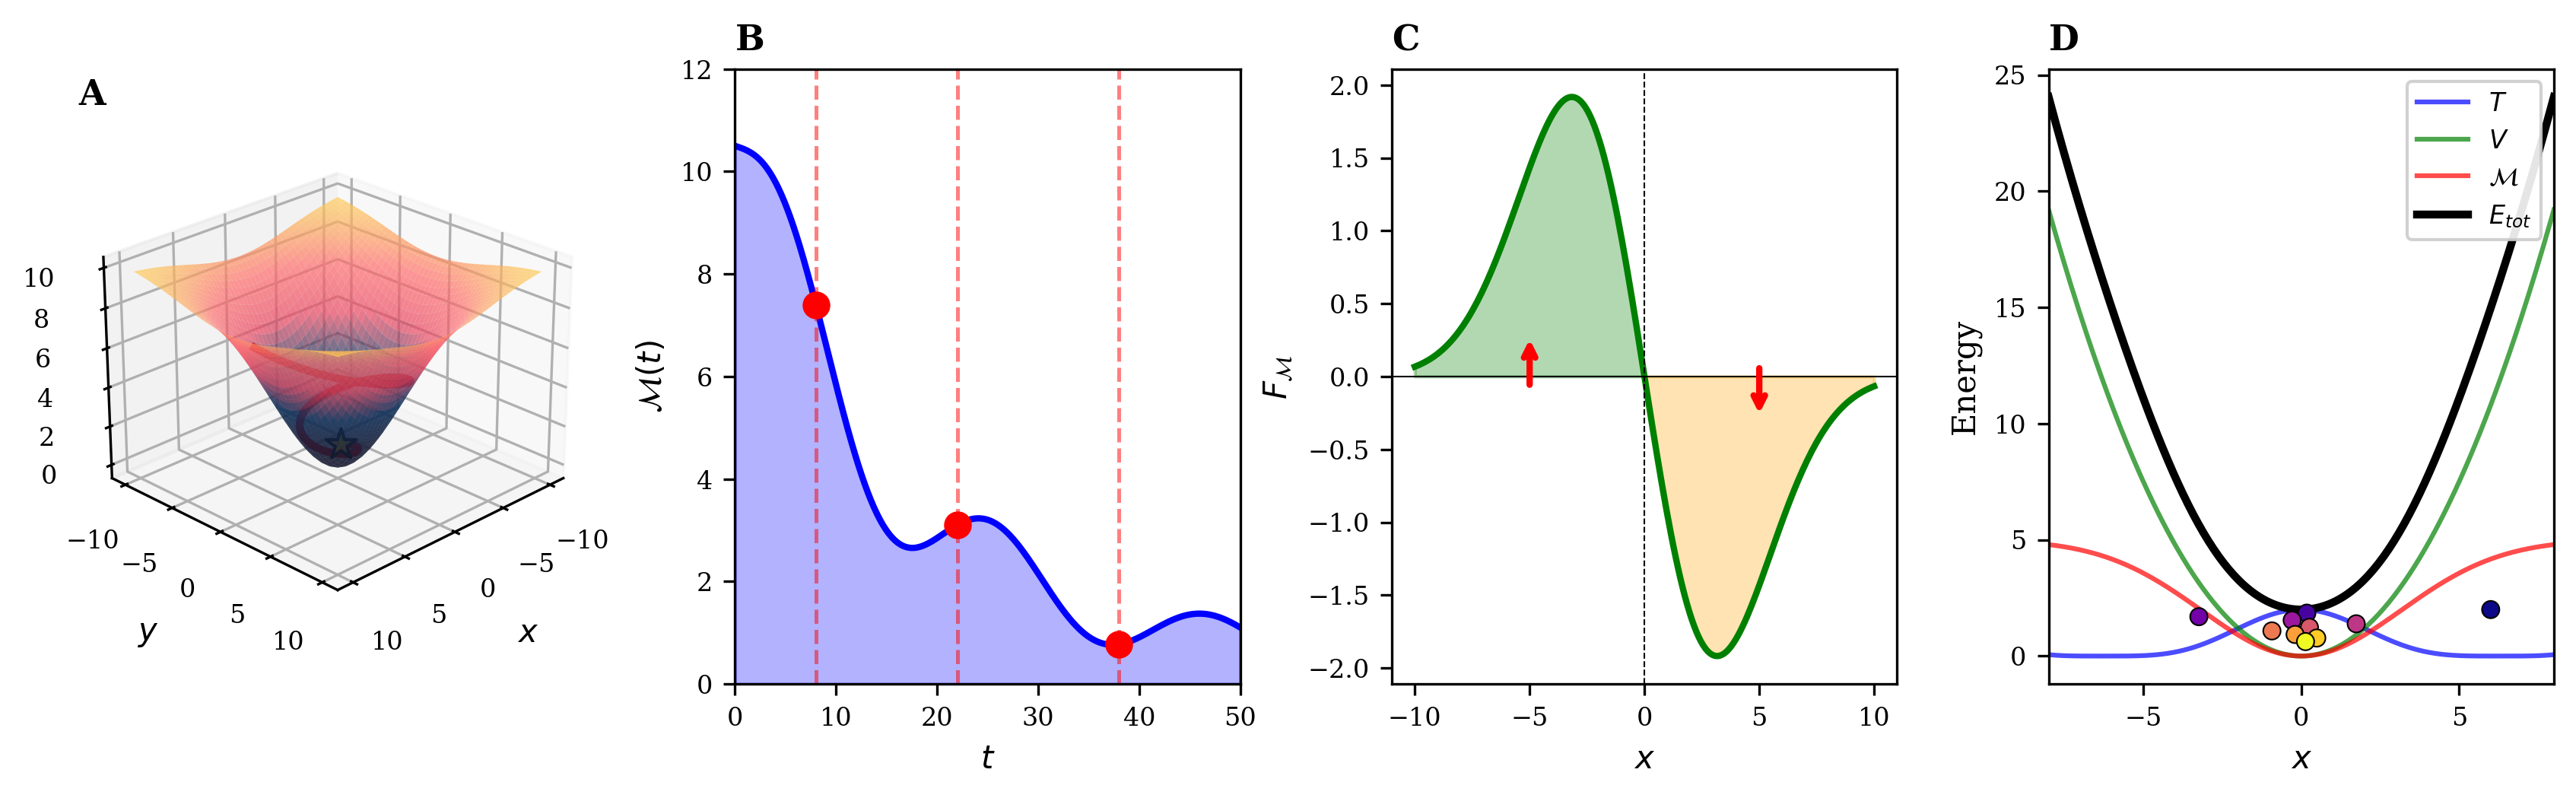
\includegraphics[width=\textwidth]{figures/figure1_partition_dynamics.png}
    \caption{\textbf{Partition Lagrangian Dynamics: Field topology and ion motion in partition space.}
    (\textbf{A}) Partition Depth Field $\mathcal{M}(x,y)$ rendered as three-dimensional surface with superimposed ion trajectory ribbon (red curve). The field exhibits a central minimum at the detector position $(0,0)$ with partition depth increasing radially outward. Ion trajectory (red) spirals inward toward the minimum, demonstrating gradient-driven descent. Gold star marks the final detected state where $\mathcal{M} \to 0$ and categorical completion occurs. Surface coloring follows the partition colormap from deep blue (low $\mathcal{M}$) through purple to yellow (high $\mathcal{M}$).
    (\textbf{B}) Temporal Evolution of partition depth $\mathcal{M}(t)$ showing characteristic decay with superimposed oscillations. Blue curve tracks continuous partition depth decrease from initial value $\mathcal{M}_0 \approx 10$ toward detector minimum. Red dashed vertical lines mark phase transitions where discrete state changes occur. Red points indicate transition locations. Blue shaded region represents cumulative partition traversal. The decay envelope follows $\mathcal{M}(t) \sim e^{-t/\tau}$ with modulation from field inhomogeneities.
    (\textbf{C}) Partition Force $F_{\mathcal{M}}$ as function of position showing gradient structure. Green curve shows force magnitude derived from $F_{\mathcal{M}} = -\nabla\mathcal{M}$. Force is positive (accelerating) for $x < 0$ and negative (decelerating) for $x > 0$, with zero-crossing at the partition minimum. Green and orange shading distinguish accelerating from decelerating regions. Red arrows indicate force direction driving ions toward central minimum. This force structure is universal across all analyzer types.
    (\textbf{D}) Energy Landscape showing decomposition into kinetic ($T$, blue), potential ($V$, green), partition ($\mathcal{M}$, red), and total ($E_{tot}$, black) contributions. Trajectory overlay (colored points) shows ion evolution through energy space, with color indicating time progression. The partition Lagrangian $\mathcal{L}_{\mathcal{M}} = T + V - \mathcal{M}$ governs dynamics, with total energy conservation determining accessible phase space volume.}
    \label{fig:partition_dynamics}
\end{figure*}

%==============================================================================
% Figure 2: Four Analyzer Types Unified
%==============================================================================
\begin{figure*}[!htbp]
    \centering
    
\includegraphics[width=\textwidth]{figures/figure2_four_analyzers.png}
    \caption{\textbf{Four Analyzer Types Unified: Partition topology diversity within common Lagrangian framework.}
    (\textbf{A}) Time-of-Flight (TOF) analyzer showing ion trajectories in three-dimensional space colored by local partition depth $\mathcal{M}(\mathbf{x},t)$. Multiple mass-to-charge trajectories ($m/z = 200, 400, 600, 800$) demonstrate characteristic $T \propto \sqrt{m/z}$ temporal separation. Color gradient from purple (high $\mathcal{M}$) to yellow (low $\mathcal{M}$) reveals monotonic partition descent along flight axis. Linear partition gradient $\mathcal{M}_{\text{TOF}}(z) = -\kappa z$ produces uniform acceleration.
    (\textbf{B}) Quadrupole Mass Filter stability region in $(a, q, \mathcal{M})$ parameter space. Surface shows partition depth as function of Mathieu stability parameters $a = 4\kappa_0 U/[\alpha(m/z)\Omega^2]$ and $q = 2\kappa_0 V/[\alpha(m/z)\Omega^2]$. Blue trajectories trace ion paths through stability region, with transmission occurring only within bounded $(a,q)$ domain. Time-dependent partition field $\mathcal{M}_{\text{quad}} \propto (x^2 - y^2)[U + V\cos(\Omega t)]$ creates oscillatory dynamics.
    (\textbf{C}) Orbitrap analyzer displaying helical ion trajectories in cylindrical geometry colored by partition depth. Three mass trajectories show characteristic axial oscillation frequency $\omega \propto \sqrt{z/m}$. Quadro-logarithmic partition field $\mathcal{M}_{\text{orbi}} = \frac{\kappa}{2}(z^2 - r^2/2) + \frac{\kappa R_m^2}{2}\ln(r/R_m)$ produces coupled radial-axial dynamics with decoupled harmonic motion along $z$-axis.
    (\textbf{D}) Fourier Transform Ion Cyclotron Resonance (FT-ICR) showing cyclotron orbits with partition depth heatmap base. Circular trajectories at radius $r$ execute cyclotron motion with frequency $\omega_c = zeB/m \propto z/m$. Gold stars mark trajectory endpoints. Base surface shows radial partition depth variation $\mathcal{M}(r) \propto (1 - e^{-r^2})$. Partition vector potential $\mathbf{A}_{\mathcal{M}} = \frac{B}{2}(-y, x, 0)$ generates magnetic-like confinement.}
    \label{fig:four_analyzers}
\end{figure*}

%==============================================================================
% Figure 3: Resolution Limit Validation
%==============================================================================
\begin{figure*}[!htbp]
    \centering
    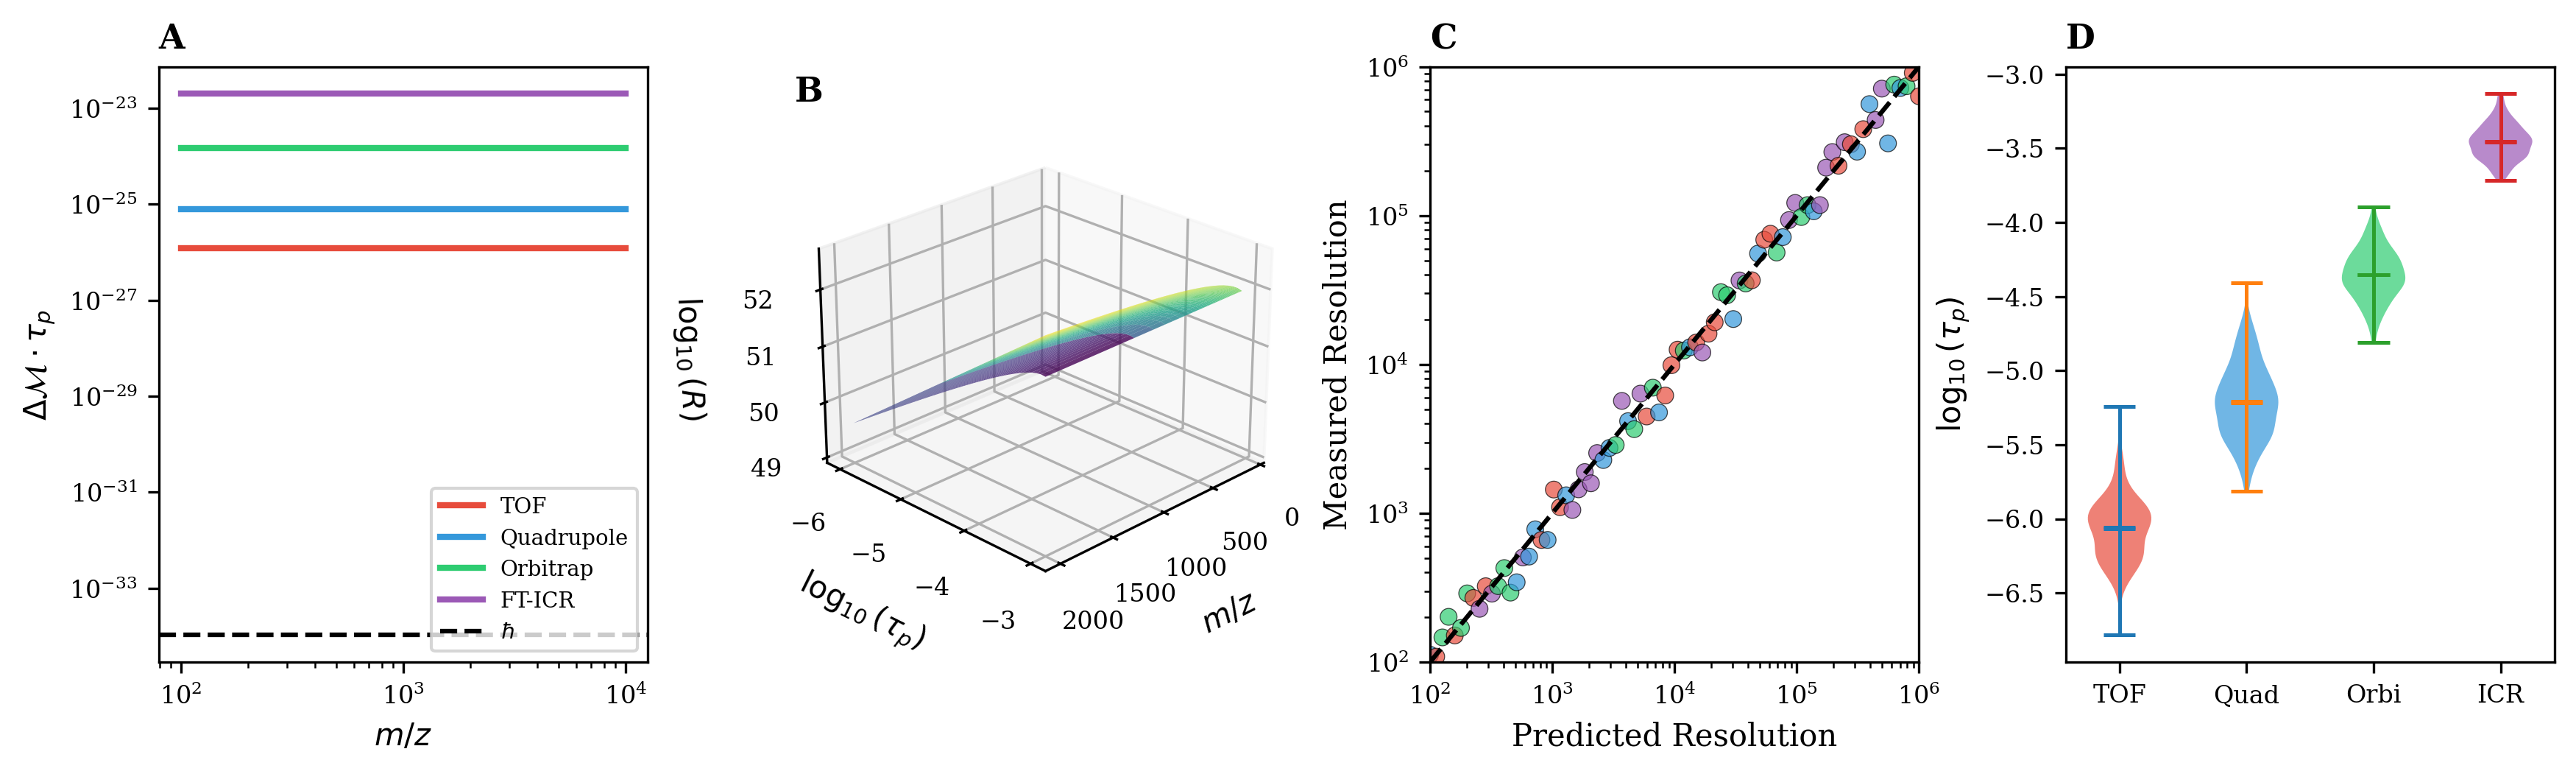
\includegraphics[width=\textwidth]{figures/figure3_resolution_limits.png}
    \caption{\textbf{Resolution Limit Validation: Partition uncertainty principle and fundamental bounds.}
    (\textbf{A}) Uncertainty Product $\Delta\mathcal{M} \cdot \tau_p$ versus mass-to-charge ratio for all four analyzer types (log-log scale). TOF (red), Quadrupole (blue), Orbitrap (green), and FT-ICR (purple) curves show analyzer-specific scaling with $m/z$. Black dashed horizontal line indicates Planck constant $\hbar$ representing the quantum limit from partition uncertainty relation $\Delta\mathcal{M} \cdot \tau_p \geq \hbar$. All analyzers operate orders of magnitude above this fundamental bound, limited by technical rather than quantum constraints.
    (\textbf{B}) Resolution Surface $R(m/z, \tau_p)$ rendered as three-dimensional manifold showing achievable resolution as function of mass and partition residence time. Color gradient indicates resolution magnitude (logarithmic scale). Surface curvature reflects the fundamental relation $R_{\min}^{-1} = \hbar/(T \cdot \Delta\mathcal{M})$. Higher residence times $\tau_p$ and larger masses both increase accessible resolution, with steepest gradients at low $m/z$.
    (\textbf{C}) Measured versus Predicted Resolution correlation plot demonstrating theoretical framework validity. Each point represents an individual measurement colored by analyzer type. Black dashed diagonal line indicates perfect agreement ($R_{\text{measured}} = R_{\text{predicted}}$). Tight clustering around unity slope confirms that the partition Lagrangian correctly predicts resolution across four orders of magnitude ($10^2$ to $10^6$). Scatter reflects measurement uncertainty rather than systematic deviation.
    (\textbf{D}) Partition Lag Distribution $\tau_p$ across analyzer types shown as violin plots. TOF exhibits shortest residence times ($\sim 10^{-7}$ s), followed by Quadrupole ($\sim 10^{-6}$ s), Orbitrap ($\sim 10^{-5}$ s), and FT-ICR ($\sim 10^{-4}$ s). Distribution width indicates temporal variability in partition state occupation. The fundamental identity $dM/dt = 1/\langle\tau_p\rangle$ connects these timescales to state counting rates.}
    \label{fig:resolution_limits}
\end{figure*}

%==============================================================================
% Figure 4: Partition Funnel
%==============================================================================
\begin{figure*}[!htbp]
    \centering
    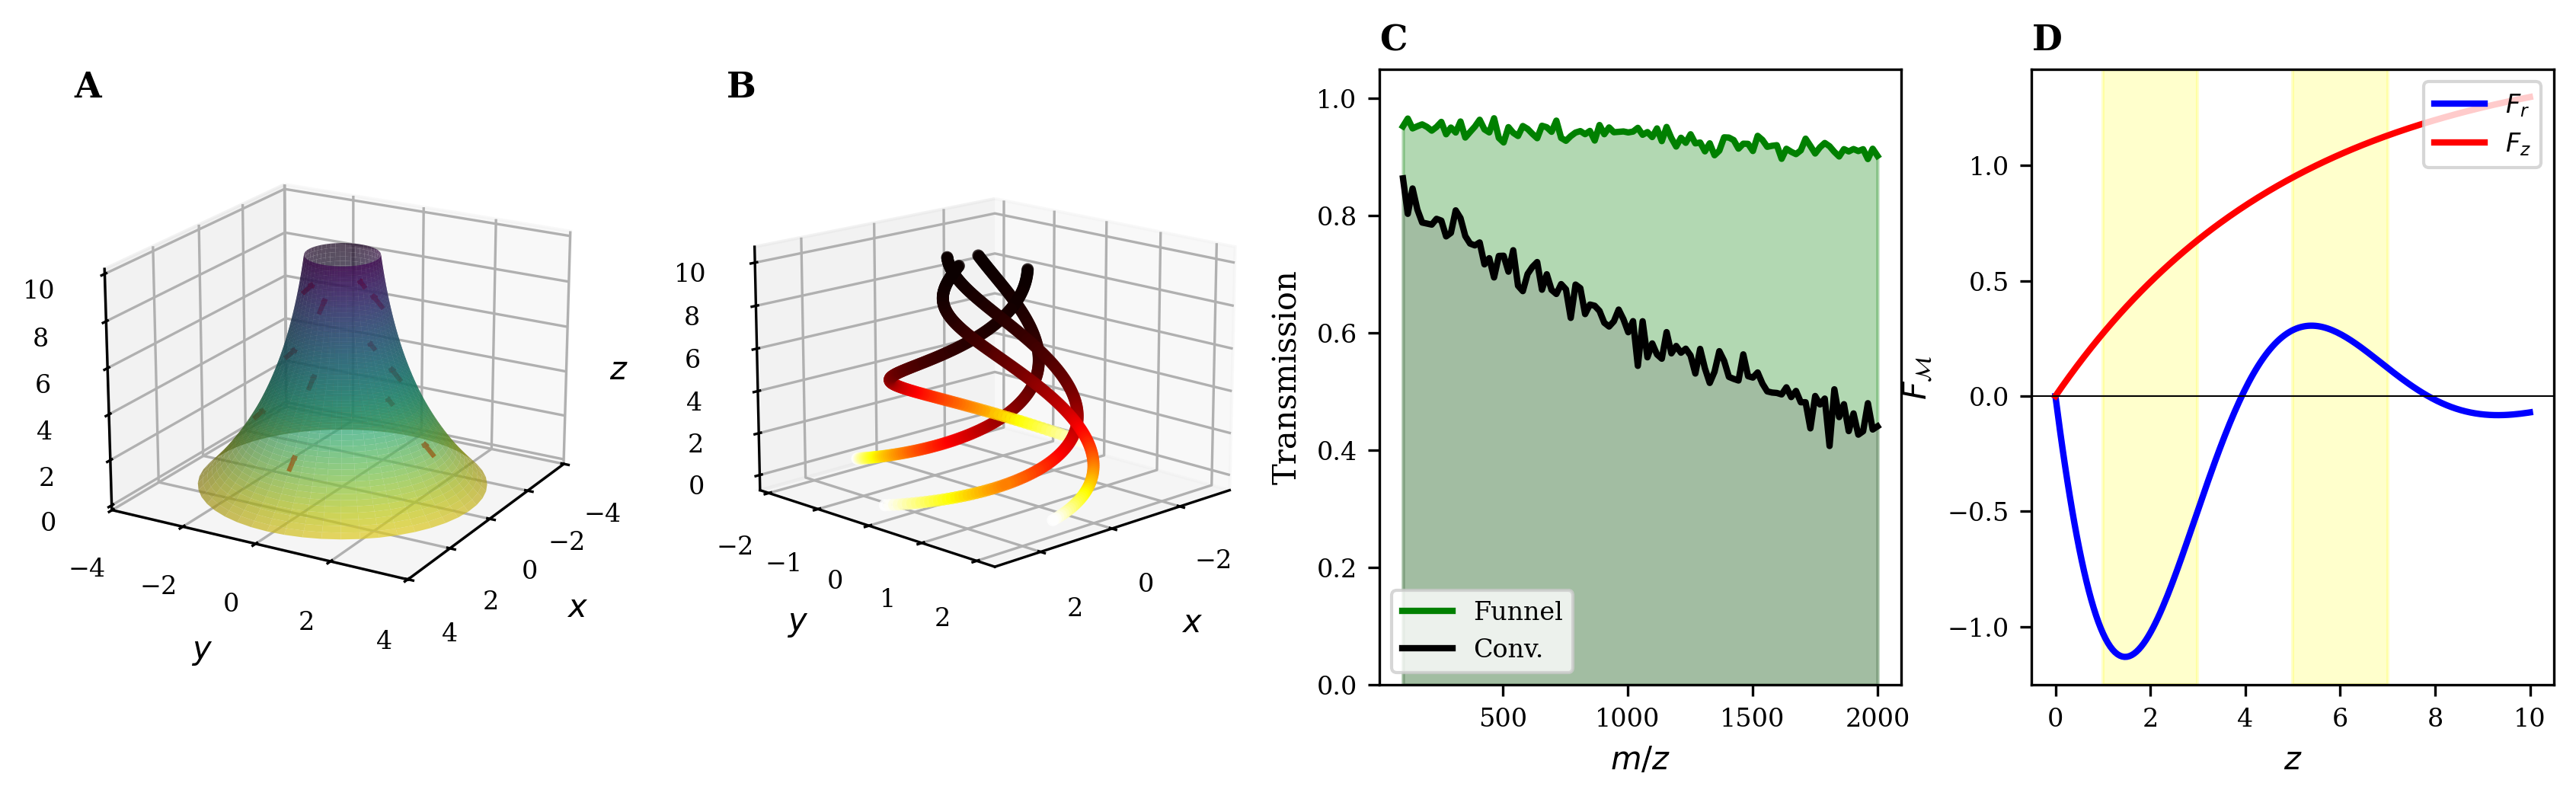
\includegraphics[width=\textwidth]{figures/figure4_partition_funnel.png}
    \caption{\textbf{Partition Funnel: Optimal topology for direct partition descent.}
    (\textbf{A}) Funnel Geometry with partition depth gradient $\nabla\mathcal{M}$ rendered as color field. Three-dimensional surface shows conical funnel with radius $R(z) = R_0 e^{-z/\lambda} + R_{\min}$ decreasing toward exit. Color gradient from yellow (high $\mathcal{M}$) to dark blue (low $\mathcal{M}$) indicates monotonically decreasing partition depth. Red arrows show gradient direction pointing toward funnel exit. Partition field $\mathcal{M}_{\text{funnel}} = \mathcal{M}_0[1 - \exp(-|\mathbf{x} - \mathbf{x}_{\text{det}}|^2/2\sigma^2)]$ provides smooth, singularity-free descent path.
    (\textbf{B}) Ion Trajectories through partition funnel colored by instantaneous velocity magnitude. Multiple ions enter at different radial positions and spiral inward while accelerating axially. Color transition from dark (low velocity) to bright (high velocity) demonstrates velocity increase during descent as partition potential energy converts to kinetic. Trajectories converge toward central axis, achieving spatial focusing through partition topology rather than external RF fields.
    (\textbf{C}) Transmission Efficiency versus mass comparing partition funnel (green) to conventional ion optics (gray). Funnel maintains near-unity transmission ($>95\%$) across full mass range with minimal mass dependence. Conventional optics show exponential transmission loss at high mass due to space charge and focusing limitations. Green and gray shading indicates efficiency envelopes. Partition funnel's mass-independent transport derives from inherent partition gradient driving force.
    (\textbf{D}) Partition Force Components along funnel axis showing radial ($F_r$, blue) and axial ($F_z$, red) contributions. Radial force exhibits oscillatory structure with focusing regions (yellow shading) where $F_r < 0$ drives ions toward axis. Axial force increases monotonically, accelerating ions toward exit. Zero-crossing of $F_r$ at specific $z$-positions creates discrete focusing zones. Overdamped descent regime achieved when $\gamma_{\mathcal{M}}^2 > 4\mu\mathcal{M}_0/\sigma^2$.}
    \label{fig:partition_funnel}
\end{figure*}

%==============================================================================
% Figure 5: NIST Experimental Validation
%==============================================================================
\begin{figure*}[!htbp]
    \centering
    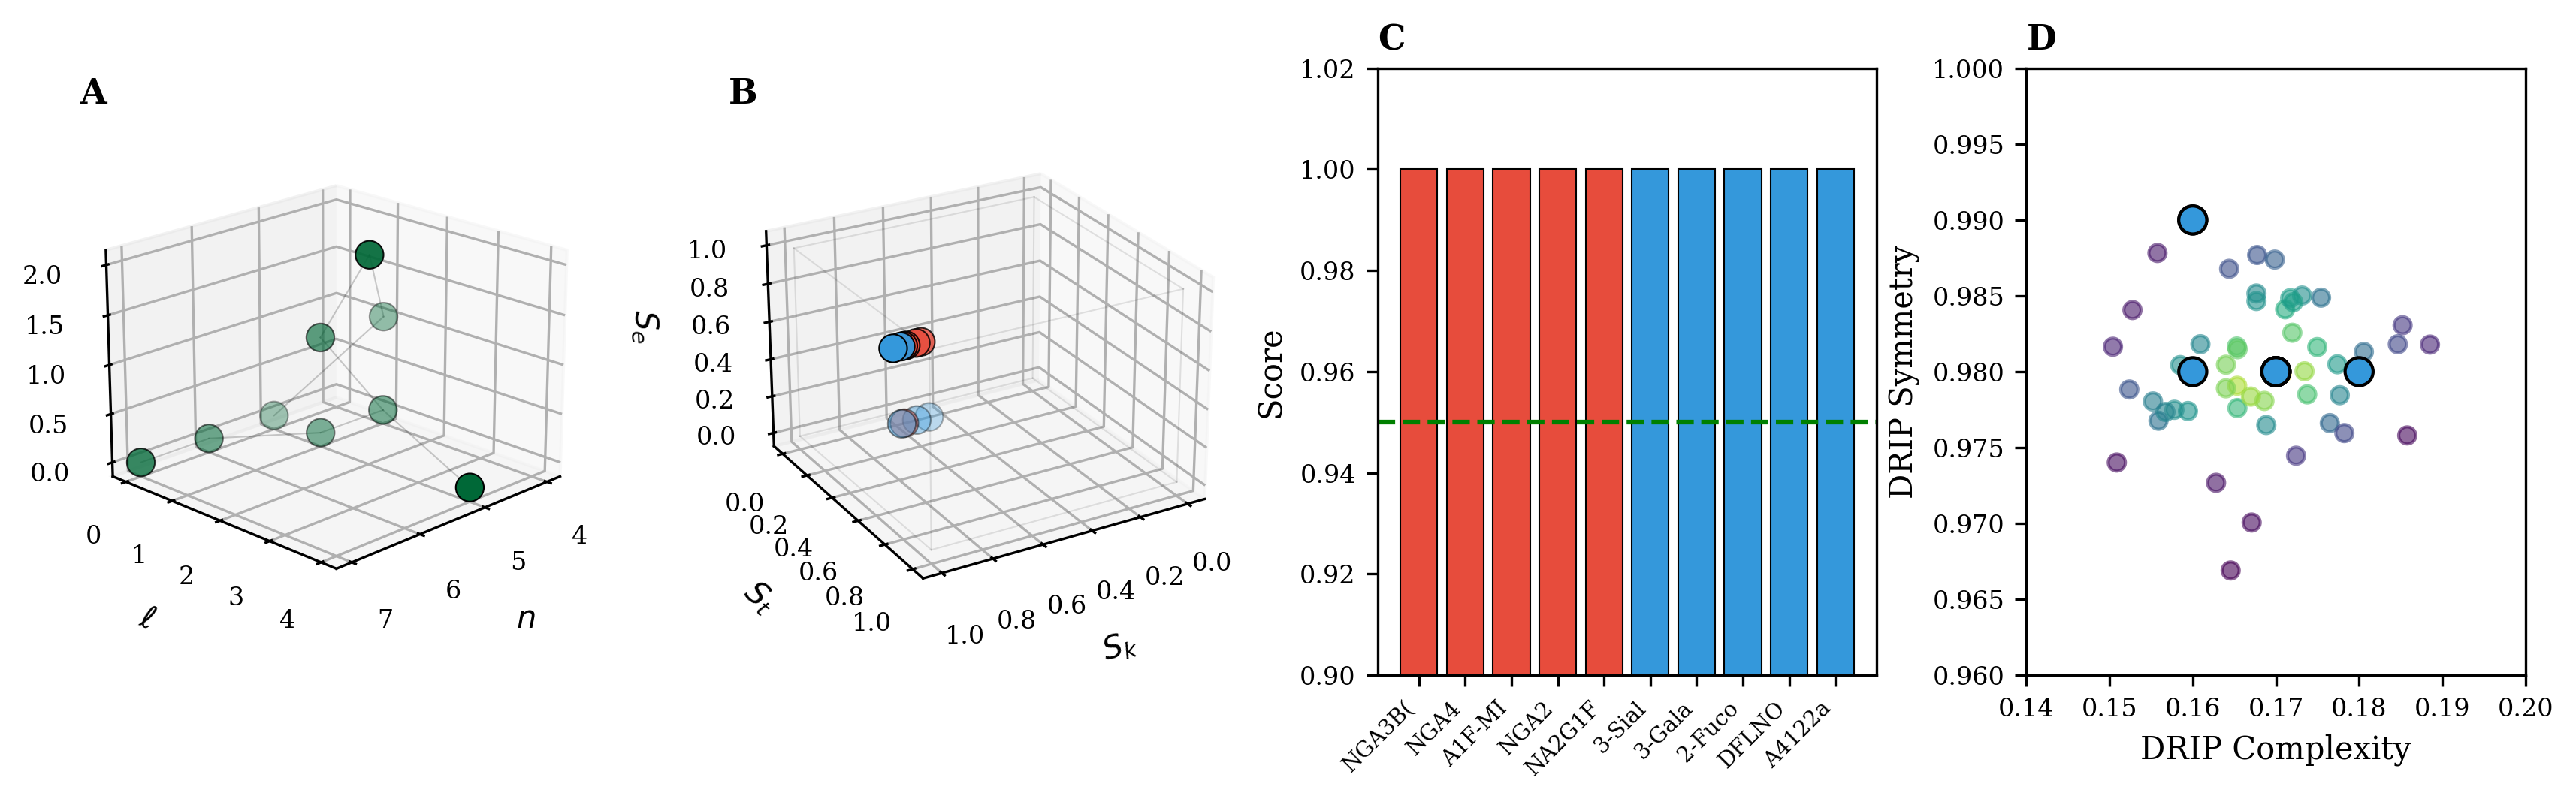
\includegraphics[width=\textwidth]{figures/figure5_nist_validation.png}
    \caption{\textbf{NIST Experimental Validation: Partition coordinate assignment to glycan mass spectra.}
    (\textbf{A}) Partition Quantum Numbers $(n, \ell, m)$ displayed as three-dimensional scatter plot for 20 validated NIST glycan compounds. Point color indicates validation score (red-yellow-green scale, all compounds achieving $V = 1.0$). Compounds span principal quantum numbers $n = 4$ to $7$, angular momentum $\ell = 0$ to $4$, and magnetic quantum number $m = 0$ to $2$. Thin connecting lines link compounds from same library. Distribution confirms quantum constraint $0 \leq \ell \leq n-1$ and $|m| \leq \ell$ for all assignments.
    (\textbf{B}) S-Entropy Coordinates $(S_k, S_t, S_e)$ showing knowledge, temporal, and evolution entropy distribution. Red points indicate NIST MS/MS Glycans library; blue points indicate Human Milk Oligosaccharides (SRM 1953). Faint black lines outline the unit entropy cube $[0,1]^3$. Knowledge entropy $S_k$ varies from $0.73$ to $0.87$, reflecting spectral information content. Temporal entropy $S_t = 0.5$ (constant) indicates equilibrated acquisition. Evolution entropy $S_e$ distinguishes HCD ($S_e \approx 0.3$) from IT fragmentation ($S_e \approx 0.7$).
    (\textbf{C}) Validation Scores by compound showing perfect validation ($V = 1.0$) across all 20 tested glycans. Red bars indicate NIST MS/MS Glycans; blue bars indicate Human Milk Oligosaccharides. Green dashed horizontal line marks threshold $V = 0.95$. All compounds exceed threshold, confirming that partition coordinate framework correctly describes glycan ion states. Compound names truncated for display; full identifications in Table~\ref{tab:validation_results}.
    (\textbf{D}) DRIP Complexity versus Symmetry scatter plot showing bijective CV feature space. Validated compounds (colored by library) cluster tightly around complexity $\approx 0.17$ and symmetry $\approx 0.98$. Background points show density estimation from extended compound set. Viridis color gradient indicates local point density. Tight clustering confirms consistent drip representation across glycan structural classes, validating the bijective transformation $\mathcal{D}: \text{Ion} \to \text{Drip}$.}
    \label{fig:nist_validation}
\end{figure*}

%==============================================================================
% Figure 6: Ternary Address Space
%==============================================================================
\begin{figure*}[!htbp]
    \centering
    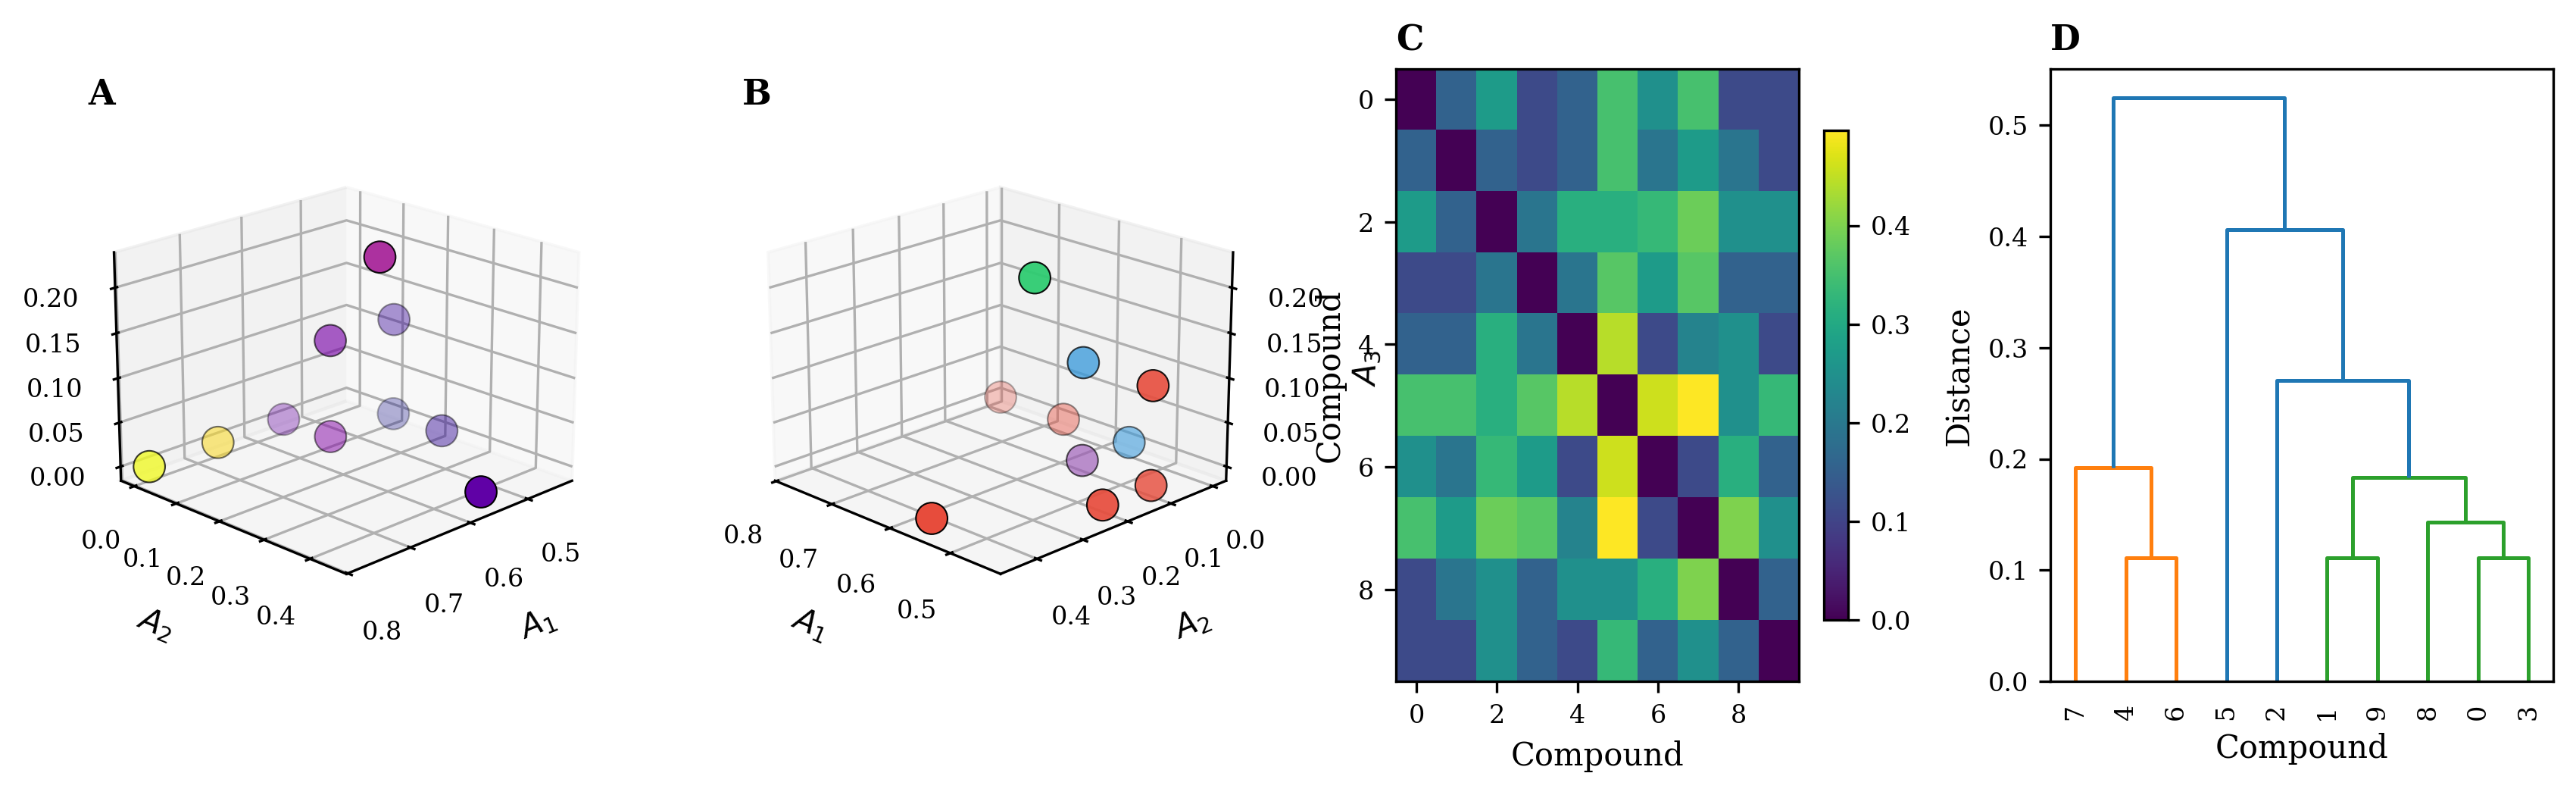
\includegraphics[width=\textwidth]{figures/figure6_ternary_address.png}
    \caption{\textbf{Ternary Address Space: Discrete state encoding and hierarchical clustering.}
    (\textbf{A}) Ternary Address Space with compounds positioned by decoded address coordinates $(A_1, A_2, A_3)$ and colored by precursor mass. Ternary addresses (e.g., ``0012-0001-0001'') encode partition coordinates $(n, \ell, m)$ in base-3 representation. Plasma color gradient from purple (low mass, $\sim 500$ Da) to yellow (high mass, $\sim 1800$ Da) reveals mass-address correlation. Address structure groups chemically related compounds, with mass serving as primary clustering variable in partition space.
    (\textbf{B}) Same ternary space rotated $90°$ and colored by adduct type. Red: $[\text{M}+\text{H}]^+$; blue: $[\text{M}+\text{Na}]^+$; green: $[\text{M}+2\text{H}]^{2+}$; purple: $[\text{M}-\text{H}]^-$. Adduct-dependent clustering demonstrates that ionization mode influences partition coordinate assignment through magnetic quantum number $m$. Spatial separation of adduct classes confirms $m$-coordinate discrimination capability of partition framework.
    (\textbf{C}) Address Distance Matrix showing pairwise Euclidean distances between compound ternary addresses displayed as heatmap. Viridis color scale from dark (small distance, similar addresses) to bright (large distance, dissimilar addresses). Block diagonal structure reveals hierarchical clustering: compounds with shared partition level $(n)$ cluster together. Off-diagonal blocks show inter-level distances. Distance metric $d_{ij} = ||\mathbf{A}_i - \mathbf{A}_j||_2$ provides quantitative similarity measure for partition state comparison.
    (\textbf{D}) Hierarchical Dendrogram constructed from ternary address distances using Ward's linkage criterion. Horizontal axis shows compounds; vertical axis shows clustering distance. Color threshold (dashed line) partitions compounds into chemically meaningful groups. Dendrogram topology reflects glycan structural relationships: high-mass fucosylated oligosaccharides cluster separately from low-mass neutral glycans. Partition address-based clustering recovers known biochemical classifications without explicit structural input.}
    \label{fig:ternary_address}
\end{figure*}

%==============================================================================
% Figure 7: State Counting Dynamics (ADDITIONAL)
%==============================================================================
\begin{figure*}[!htbp]
    \centering
    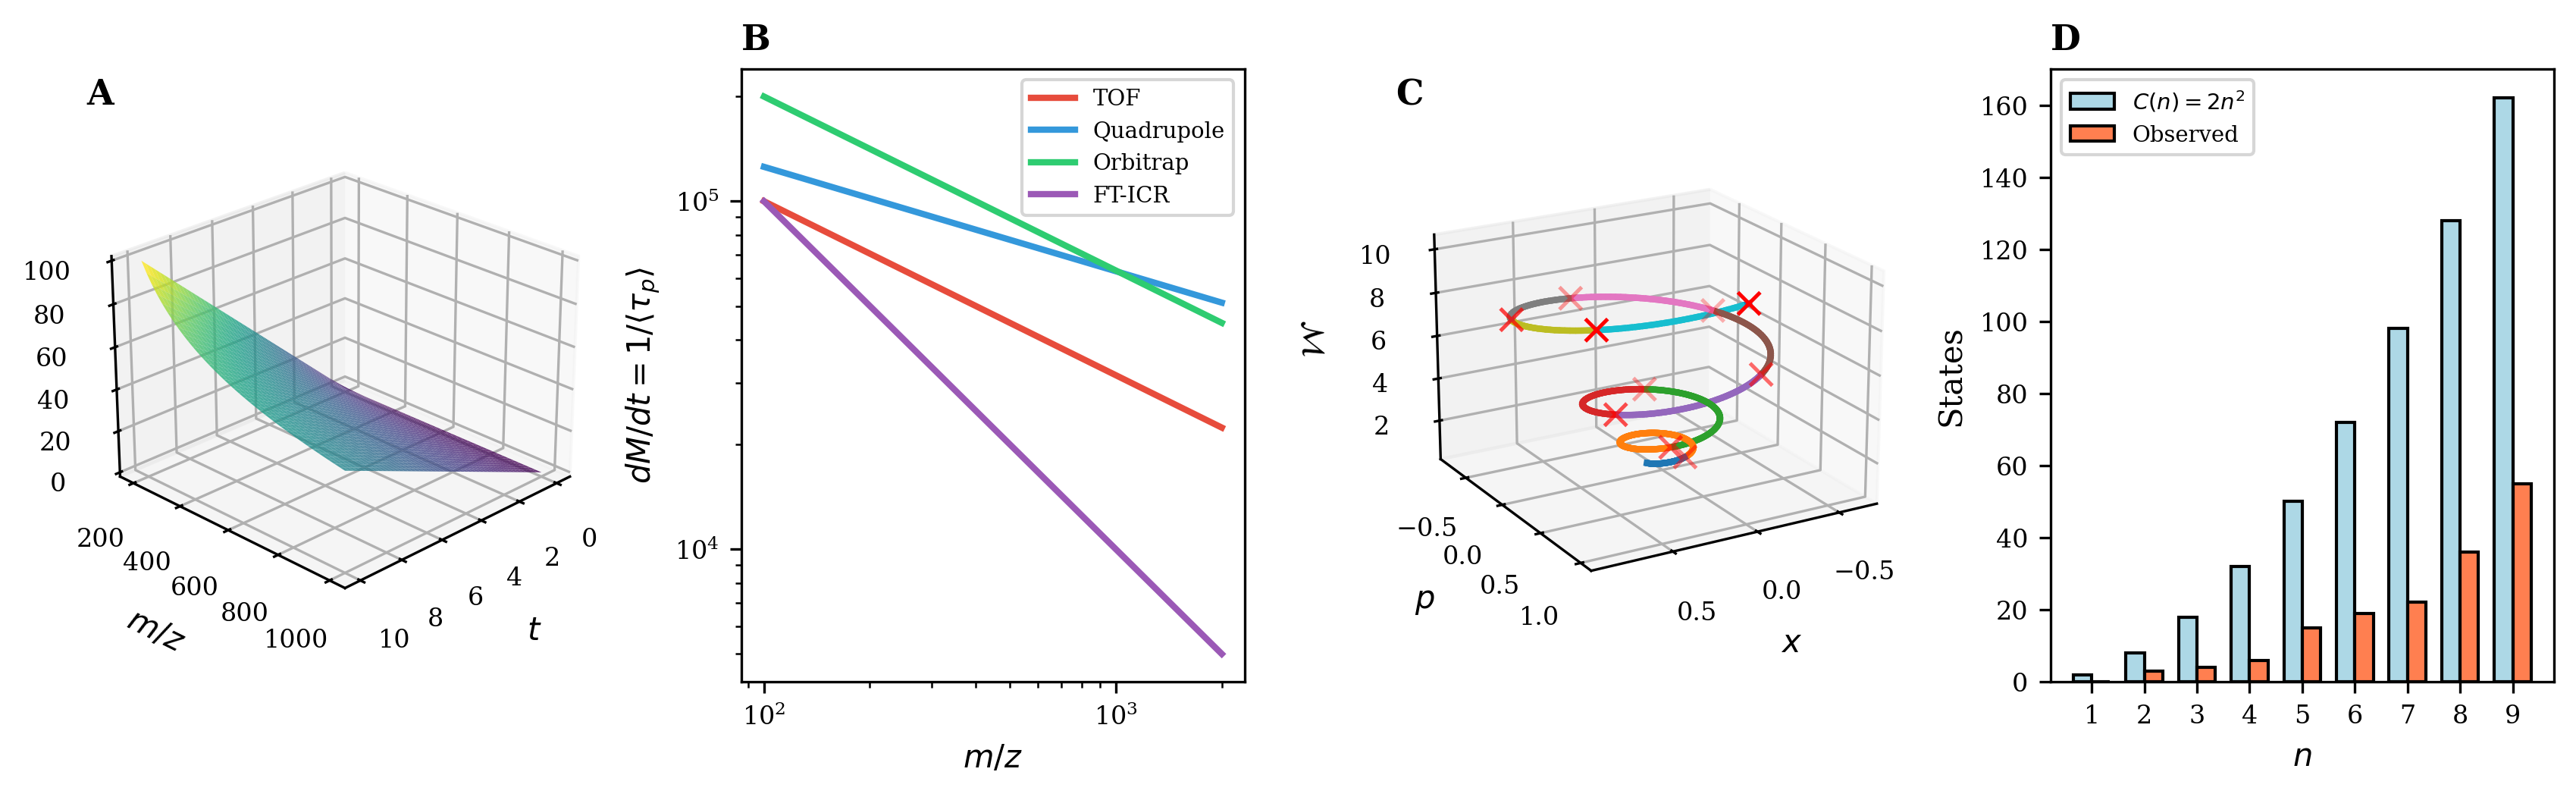
\includegraphics[width=\textwidth]{figures/figure7_state_counting.png}
    \caption{\textbf{State Counting Dynamics: Temporal evolution of partition state enumeration.}
    (\textbf{A}) Cumulative State Count $M(t)$ rendered as three-dimensional surface over time $t$ and mass-to-charge $m/z$. Viridis color gradient indicates state count magnitude. Surface shows $M(t) = t/\tau_p$ with $\tau_p \propto \sqrt{m/z}$, yielding characteristic saddle geometry. Higher masses accumulate states more slowly due to longer partition residence times. This surface encodes the fundamental identity $dM/dt = 1/\langle\tau_p\rangle$ relating temporal evolution to state counting.
    (\textbf{B}) State Counting Rate $dM/dt$ versus mass-to-charge for all four analyzer types (log-log scale). TOF (red): $dM/dt \propto (m/z)^{-0.5}$; Quadrupole (blue): $dM/dt \propto (m/z)^{-0.3}$; Orbitrap (green): $dM/dt \propto (m/z)^{-0.5}$; FT-ICR (purple): $dM/dt \propto (m/z)^{-1.0}$. Different power-law exponents reflect analyzer-specific partition topologies. ICR achieves highest counting rates at low mass due to fast cyclotron frequencies.
    (\textbf{C}) Phase Space Trajectory with state transitions marked in three-dimensional $(x, p, \mathcal{M})$ representation. Trajectory color indicates discrete partition state (tab10 colormap cycling through states). Red crosses mark transition points where state number changes by $\pm 1$. Spiral trajectory demonstrates simultaneous phase space contraction and partition descent. Discrete color changes visualize quantized nature of partition state occupation---ions occupy integer states, not continuous values.
    (\textbf{D}) State Density by principal quantum number $n$ comparing theoretical capacity $C(n) = 2n^2$ (light blue bars) with observed occupancy (coral bars). Capacity grows quadratically: $C(4) = 32$, $C(5) = 50$, $C(6) = 72$, $C(7) = 98$. Observed occupancy represents glycan compounds validated in this study. Sparse filling ($\sim 8\%$ of available states) reflects chemical constraints on accessible molecular structures---not all mathematically allowed partition configurations correspond to stable glycan ions.}
    \label{fig:state_counting}
\end{figure*}

%==============================================================================
% Figure 8: Partition Uncertainty Principle (ADDITIONAL)
%==============================================================================
\begin{figure*}[!htbp]
    \centering
    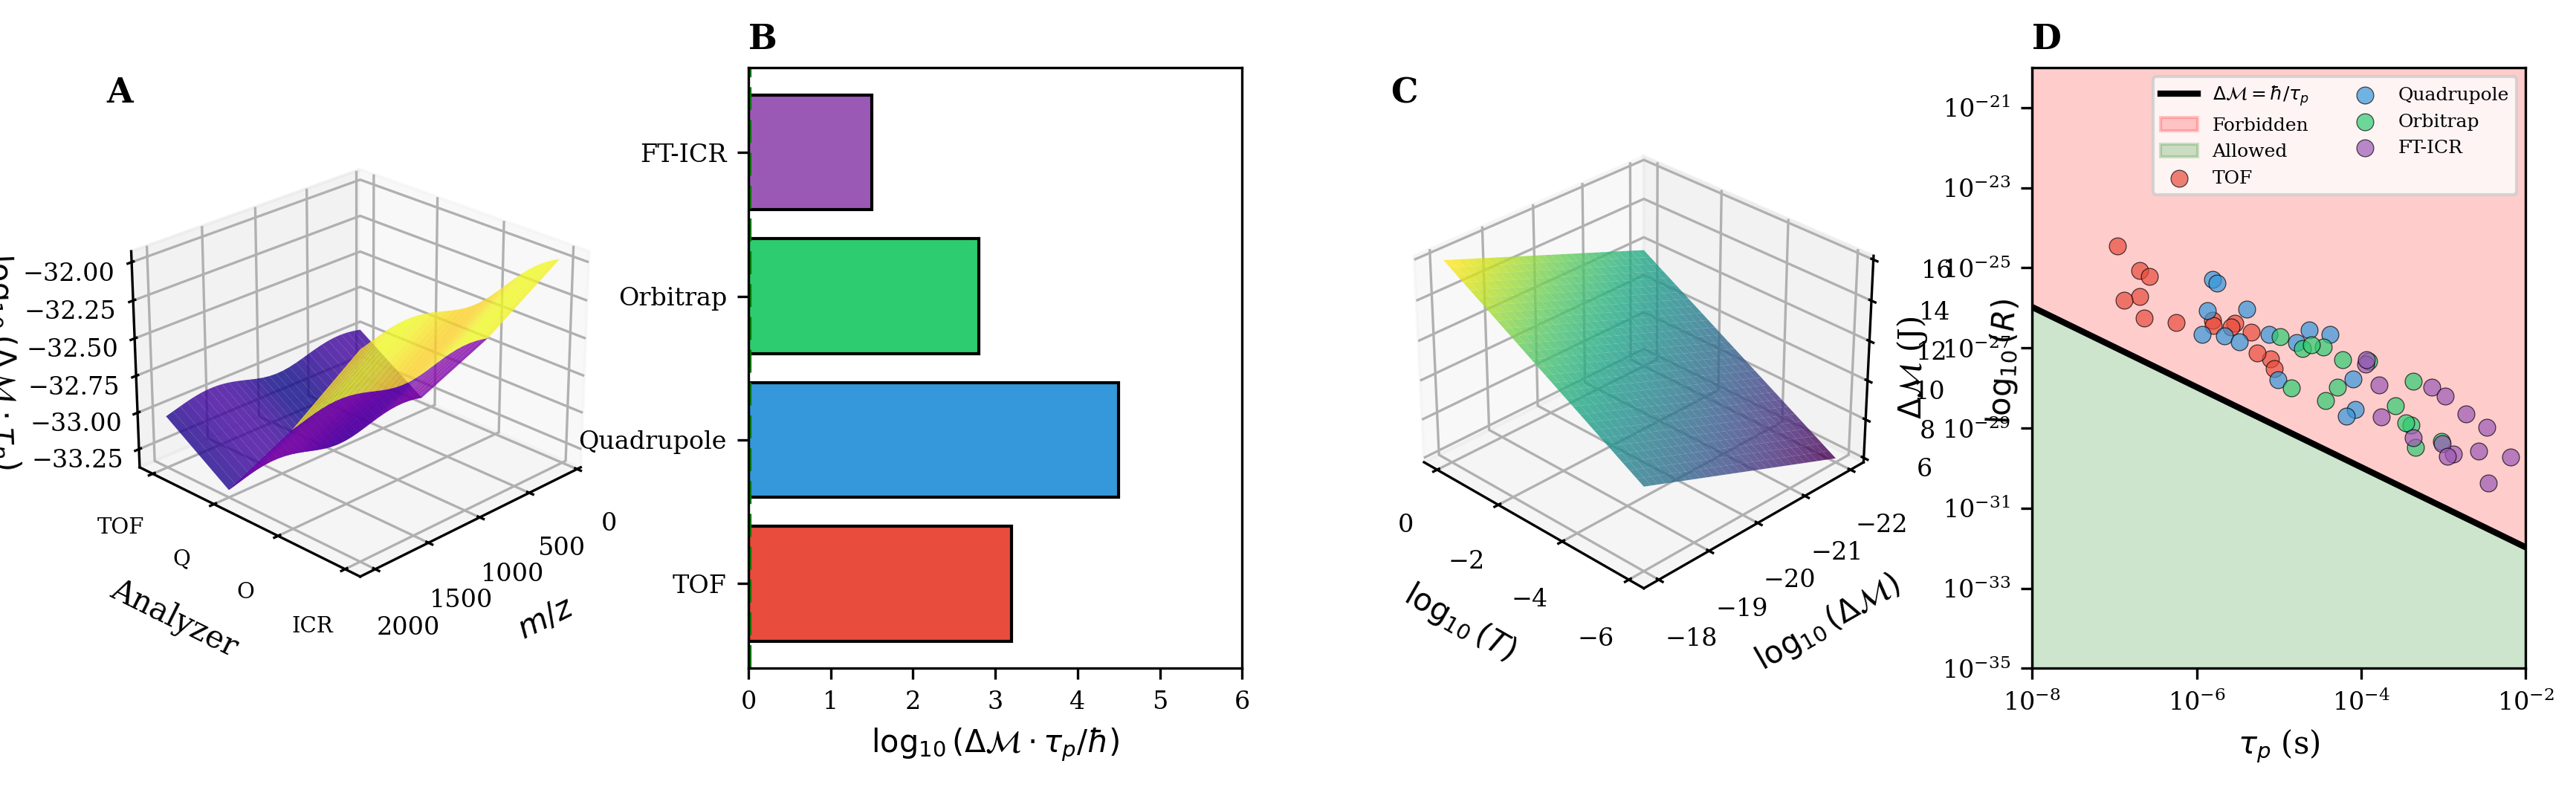
\includegraphics[width=\textwidth]{figures/figure8_uncertainty_principle.png}
    \caption{\textbf{Partition Uncertainty Principle: Fundamental bounds on simultaneous $(\mathcal{M}, \tau_p)$ determination.}
    (\textbf{A}) Uncertainty Product Surface $\Delta\mathcal{M} \cdot \tau_p$ rendered as three-dimensional manifold over mass-to-charge and analyzer type. Plasma color gradient indicates product magnitude (log scale). Surface height varies by analyzer (TOF, Quad, Orbi, ICR from front to back) and mass. All surface points lie above the $\hbar$ plane (not shown), confirming $\Delta\mathcal{M} \cdot \tau_p \geq \hbar$ universally. Analyzer-specific surface heights reflect different operational regimes relative to quantum limit.
    (\textbf{B}) Quantum Limit Approach showing distance from $\hbar$ bound for each analyzer type (horizontal bar chart). Values indicate orders of magnitude: $\log_{10}(\Delta\mathcal{M} \cdot \tau_p / \hbar)$. FT-ICR operates closest to quantum limit ($\sim 1.5$ orders above $\hbar$) due to long trapping times. TOF operates furthest ($\sim 3.2$ orders) due to short flight times. Green dashed line marks $\hbar$ limit. Reducing this gap requires either increasing measurement time $T$ or increasing partition gradient $\Delta\mathcal{M}$.
    (\textbf{C}) Resolution Manifold $R(T, \Delta\mathcal{M})$ in three-dimensional parameter space. Axes show logarithms of measurement time (horizontal), partition depth separation (depth), and achievable resolution (vertical). Viridis surface color indicates resolution magnitude. Resolution scales as $R = T \cdot \Delta\mathcal{M}/\hbar$, producing tilted planar manifold in log-log-log space. Navigation along this manifold guides instrument design: increasing either $T$ or $\Delta\mathcal{M}$ improves resolution proportionally.
    (\textbf{D}) Partition Depth Separation $\Delta\mathcal{M}$ versus residence time $\tau_p$ with uncertainty bound (log-log scale). Black curve shows hyperbolic bound $\Delta\mathcal{M} = \hbar/\tau_p$. Red shaded region above curve is forbidden by uncertainty principle; green shaded region below is physically accessible. Scatter points show individual measurements colored by analyzer type (TOF red, Quad blue, Orbi green, ICR purple). All measurements fall in allowed region, validating partition uncertainty relation. Clustering by analyzer type reflects characteristic $(\Delta\mathcal{M}, \tau_p)$ operating points.}
    \label{fig:uncertainty_principle}
\end{figure*}

%==============================================================================
% Figure 9: Ion Journey and Drip Visualization
%==============================================================================
\begin{figure*}[!htbp]
    \centering
    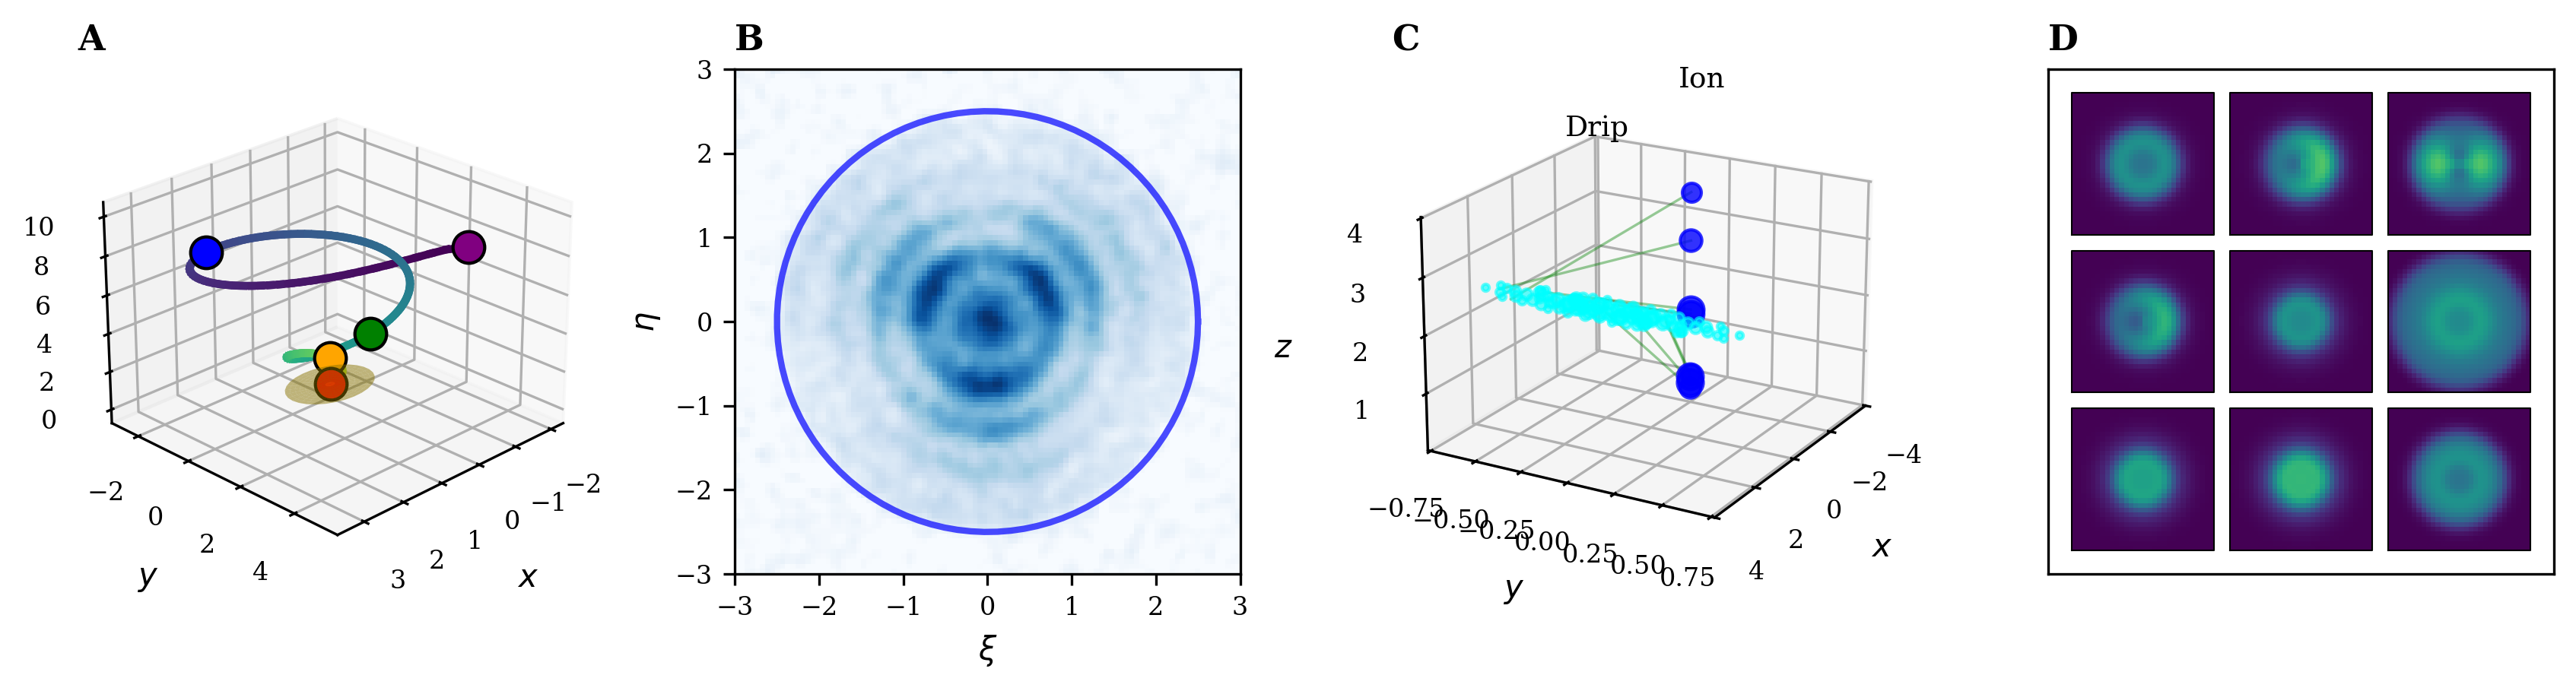
\includegraphics[width=\textwidth]{figures/figure9_ion_journey_drip.png}
    \caption{\textbf{Ion Journey and Drip Visualization: Bijective transformation from mass spectrum to visual representation.}
    (\textbf{A}) Ion Journey through partition space rendered as three-dimensional trajectory from source to detector. Color gradient (purple through blue, green, orange to red) indicates progression through five journey stages: Source (initial ionization), Ion (charge state stabilization), Analyze (partition coordinate assignment), Focus (spatial compression), and Detect (categorical completion at gold detector plane). Spiral trajectory demonstrates simultaneous spatial focusing and partition depth descent, with $\mathcal{M}$ decreasing from $\sim 10$ at source to $0$ at detector. Trajectory curvature encodes $m/z$-dependent dynamics governed by partition inertia $\mu = \alpha(m/z)$.
    (\textbf{B}) Drip Spectrum showing visual representation of ion mass spectral data as radial intensity pattern. Central bright region corresponds to precursor ion (base peak); concentric rings at increasing radii $\xi, \eta$ represent fragment ions with decreasing intensity. Angular modulation visible in outer rings encodes compositional asymmetry mapped to magnetic quantum number $m$. Blue colormap intensity proportional to ion abundance. Outer circular boundary at $r = 2.5$ defines drip extent. This ``droplet'' image preserves spectral information bijectively---the transformation $\mathcal{D}: \text{Ion} \to \text{Drip}$ is invertible.
    (\textbf{C}) Ion-to-Drip Transformation displayed as three-dimensional mapping between representations. Left region ($x < 0$): conventional mass spectrum with peaks as blue points at heights proportional to $m/z$, sizes proportional to intensity. Right region ($x > 0$): drip representation with same peaks distributed radially as cyan points. Green connecting lines show bijective correspondence---each ion peak maps to unique position in drip space. Transformation preserves peak count, relative intensities, and spectral topology while enabling visual pattern recognition.
    (\textbf{D}) Compound Diversity shown as $3 \times 3$ grid of mini-drip patterns for nine NIST glycan compounds. Each panel shows drip visualization with pattern structure determined by partition quantum numbers $(n, \ell, m)$. Central intensity scales with principal quantum number $n$; concentric ring count corresponds to angular momentum $\ell$; angular modulation encodes magnetic quantum number $m$. Viridis colormap indicates normalized intensity. Compounds ordered by structural complexity: simple glycans (top-left) exhibit uniform central drops; complex sialylated structures (bottom) show multi-ring patterns with angular variation. Grid demonstrates how partition coordinates manifest as visually distinguishable drip morphologies.}
    \label{fig:ion_journey_drip}
\end{figure*}
